\chapter{Promisingness: 새로운 축은 정말 최선인가}
\label{STC-S10}

질문은 ``sleep이라는 이름이 흥미로운가''가 아니라, 동일한 wake evidence와 future query를 주었을 때
deferred transformation이 long context, RAG, periodic refresh, model editing, wake TTT보다 더 나은
lifetime frontier를 만드는가다. 여기서 frontier는 quality만이 아니라 total retained state, later-wake
cost, freshness, delete, rollback, wake-SLA까지 포함한다.

\section{현재 증거가 지지하는 범위}

공개 industry evidence는 external-memory sleep과 background synthesis에서 가장 강하며, 광범위한
per-user foundation-weight sleep에서는 그렇지 않다.\claim{STC-C038}
\autocite{srcstc0052,srcstc0059,srcstc0063,srcstc0065} 이는 external 방식이 영원히 우월하다는
뜻이 아니라, 이미 배포된 lifecycle과 아직 연구-scale인 parametric mechanism을 구분한다는 뜻이다.

Broad parametric sleep은 continual retention, rollback, deletion, security, fleet serving economics를
동시에 입증하지 못했다.\claim{STC-C039} ``Language Models Need Sleep''은 self-modification과
consolidation의 direct evidence지만 연구 규모의 method result이고, sequential fact learning은 weight에
남은 정보가 normal behavior에서 접근 불가능해질 수 있음을 보여 준다. External memory도 poisonable하기
때문에 단순히 외부에 두면 문제가 끝나는 것은 아니다.\autocite{srcstc0021,srcstc0036,srcstc0042}

\begin{figure}[htbp]
  \centering
  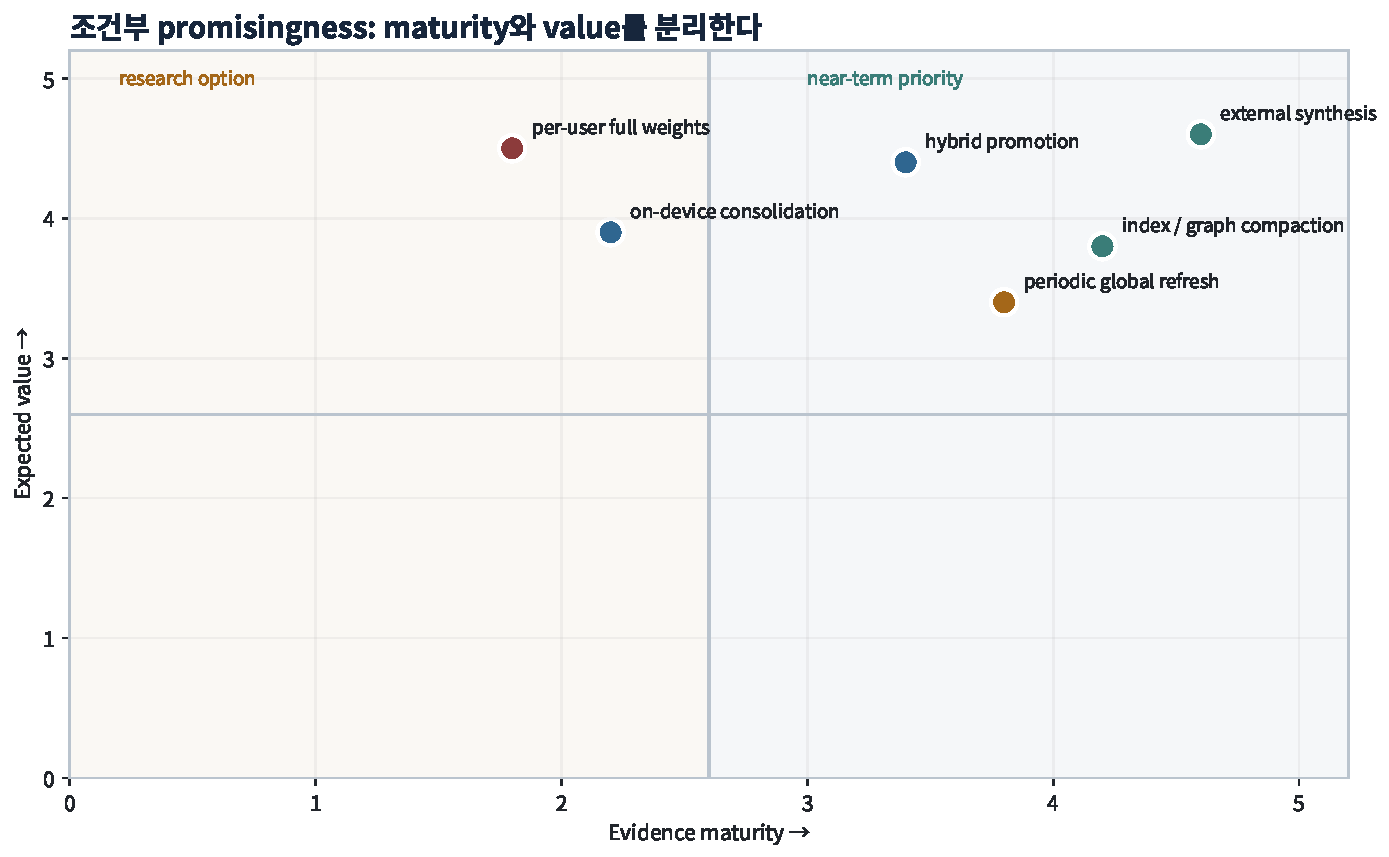
\includegraphics[width=0.96\textwidth]{figures/stc-f005.pdf}
  \caption{Evidence maturity와 expected value를 분리한 conditional verdict. 오른쪽 위로 갈수록 현재
  증거와 잠재 가치가 함께 높다. Parametric sleep은 잠재 가치가 커도 성숙도가 낮은 연구 bet로 남는다.}
  \stcfigure{STC-F005}
  \figsource{Original synthesis; SRC-STC-0052, SRC-STC-0063, SRC-STC-0021}{External synthesis, learned writer, adapter promotion, broad weight update를 성숙도와 기대 가치의 두 축에 배치한 산점도.}
  \label{fig:conditional-promisingness}
\end{figure}

가장 신뢰할 중기 구조는 auditable external system-of-record에 원 증거를 남기고, stable하고
high-reuse인 일부만 reversible adapter 또는 bounded parametric state로 승격하는 hybrid다.
\claim{STC-C040}\autocite{srcstc0027,srcstc0030,srcstc0052,srcstc0066}
Parametric artifact는 기억의 원장이 아니라 serving을 위한 compiled cache로 취급한다. Base model,
consent, evidence validity가 바뀌면 external source에서 다시 만들 수 있어야 한다.

\section{여섯 개의 핵심 verdict}

\begin{longtable}{L{0.16\textwidth} L{0.19\textwidth} L{0.28\textwidth} L{0.22\textwidth}}
\caption{핵심 주장별 조건부 verdict와 반증 조건}\label{tab:promisingness-verdicts}\\
\toprule
Claim & Verdict & 근거가 허용하는 범위 & Confidence를 낮출 관측 \\
\midrule
\endfirsthead
\toprule
Claim & Verdict & 근거가 허용하는 범위 & Confidence를 낮출 관측 \\
\midrule
\endhead
새 scaling phase인가 & functional level에서 yes & release-time training도 current-query reasoning도 아닌 durable later-wake state budget & matched synchronous maintenance와 차이가 전혀 없음 \\
mainstream인가 & lifecycle은 likely, 명칭·parametric form은 uncertain & persistent agent의 background synthesis/validation & 주요 platform이 scheduled transform을 채택하지 않음 \\
long context의 최선인가 & generally no & predictable high-reuse query에서 compile break-even 가능 & high reuse에서도 quality/cost crossover 없음 \\
continual learning 해결인가 & useful phase, solution theorem은 아님 & replay·regularization·isolation을 실행할 시간 경계 제공 & repeated cycle에서 빠른 capacity knee \\
parametric이 external보다 우월한가 & content-dependent & stable skill은 compile, volatile exact fact는 external & 단일 medium이 모든 축에서 지배 \\
device opportunity인가 & workload는 yes, 제품 claim은 별도 검토 & version, lineage, compaction, mixed read/write가 새 trace 생성 & 실제 trace가 작은 metadata job에 머묾 \\
\bottomrule
\end{longtable}

\section{문제별 strongest alternative와 sleep의 조건}

\textbf{One-off long context.} 한 번 읽고 답하는 문서는 FlashAttention 기반 long context 또는 RAG가
정확한 evidence와 citation을 보존한다. Sleep compilation은 query 전에 비용을 내고 정보 손실과
staleness를 추가하므로 reuse 예측이 없으면 열세다.

\textbf{Mutable factual memory.} Temporal graph와 versioned retrieval이 현재값, 과거값, supersession,
delete를 직접 표현한다. Parametric write가 경쟁하려면 normal-query reachability와 exact reversal을
추가로 증명해야 한다.

\textbf{Repeated procedure와 strategy.} 동일 repository, tool, enterprise procedure가 반복되면
retrieval/context token과 reasoning latency를 매번 지불한다. 이때 background synthesis, learned
strategy memory, adapter compilation이 유망하다. 다만 exact-repeat가 아니라 held-out semantic transfer로
효과를 측정해야 한다.\autocite{srcstc0043,srcstc0054}

\textbf{Global common knowledge.} 사용자별 sleep보다 centralized continued pre-training과 periodic
refresh가 더 넓게 amortize된다. STC가 이기려면 central release cadence보다 빠른 local adaptation 또는
공유할 수 없는 private evidence라는 조건이 필요하다.

\textbf{On-device personalization.} Idle window, privacy, intermittent connectivity는 sleep scheduling과
잘 맞지만 thermal, battery, write endurance, recovery state까지 포함한 측정이 없다면 가능성만 말할 수
있다. Cloud 비용을 device 비용으로 옮긴 것을 효율 향상으로 세면 안 된다.

\section{Workload별 판단}

\begin{table}[htbp]
\centering
\caption{Workload별 expected value와 현재 evidence maturity}
\label{tab:workload-promisingness}
\begin{tabularx}{\textwidth}{L{0.25\textwidth} C{0.14\textwidth} C{0.18\textwidth} Y}
\toprule
Workload & 가치 & 성숙도 & 현재 추천 \\
\midrule
multi-year personal assistant & 높음 & E4 external / E1 parametric & external synthesis 우선 \\
enterprise procedure/coding & 매우 높음 & E2--E3 & external strategy + selective adapter 실험 \\
one-off document QA & 낮음--중간 & E5 baseline & long context/RAG 우선 \\
recurring technical corpus & 높음 & E2 & reuse sweep 뒤 compile \\
universal current facts & 중간 & E5 refresh/RAG & global refresh + retrieval \\
private local adaptation & 높음 & E1 & thermal/endurance 포함 pilot \\
high-churn profile & external 높음 & E4 external & versioned external only \\
robotics/autonomy & 높음 & E1--E2 & safety-gated domain sleep \\
\bottomrule
\end{tabularx}
\end{table}

\section{의사결정 규칙}

새 evidence $e$를 destination $j$로 compile하는 decision은 단순 score가 아니라 최소 다목적 제약이다.

\begin{equation}
\text{promote}(e,j) \Longleftrightarrow
\begin{cases}
\widehat R_v(e)\,\Delta U_j(e) > C_{life}(e,j),\\
P(\text{valid at reuse}) \ge \tau_v,\\
\text{delete/rollback/compatibility gates pass},\\
\Delta U_{old},\Delta U_{safety} \ge -\epsilon.
\end{cases}
\end{equation}

하나라도 모르면 external에 남기는 것이 기본값이다. 이 규칙은 STC를 특별 대우하지 않는다. External
summary도 원본을 버리거나 false merge를 만들 수 있으므로 같은 validation과 lineage gate를 통과해야
한다.

\begin{keypoint}[Promisingness verdict]
Sleep-time compute은 하나의 universal method가 아니라 미래 wake를 위해 비용을 선불 지불하는 lifecycle
class다. 현재 가장 promising한 부분은 external background transformation과 learned memory policy이고,
가장 high-upside지만 불확실한 부분은 selective reversible parametric promotion이다. Continuous per-user
base-weight update는 현재 strongest default가 아니다.
\end{keypoint}
